%%
%% CS 502 Final Report — Spring 2026
%% Systematic Benchmarking of Multiple Sequence Alignment Algorithms
%% Anand Meena & Shruthi Kodati, University of Illinois at Chicago
%%
%% Force natbib into numeric mode BEFORE the class loads it
\PassOptionsToPackage{numbers,sort&compress}{natbib}
\documentclass[unnumsec,webpdf,contemporary,large]{oup-authoring-template}

%% ── Packages ──────────────────────────────────────────────────────────────────
\usepackage[T1]{fontenc}
\usepackage{graphicx}
\usepackage{booktabs}
\usepackage{multirow}
\usepackage{amsmath}
\usepackage{hyperref}
%% natbib is loaded by oup-authoring-template.cls — force numeric mode via public API
\setcitestyle{numbers,open={[},close={]}}
\usepackage{microtype}

\graphicspath{{figures/}}

%% ── Style overrides ───────────────────────────────────────────────────────────
%% Make subsection headings visually bold (use \bfseries explicitly)
\makeatletter
\def\subsecsize{%
  \fontsize{10bp}{12}\bfseries\selectfont\leftskip0pt\rightskip0pt plus1fill}
\makeatother

%% ── Journal / article metadata ───────────────────────────────────────────────
\journaltitle{Bioinformatics}
\copyrightyear{2026}
\pubyear{2026}
\firstpage{1}

%% ── Title ─────────────────────────────────────────────────────────────────────
\title[MSA Benchmark]{Systematic Benchmarking of Multiple Sequence Alignment
    Algorithms on Structurally-Informed Reference Datasets}

%% ── Authors ───────────────────────────────────────────────────────────────────
\author[1]{Anand Meena}
\author[1]{Shruthi Kodati}

\address[1]{%
  \orgdiv{Department of Computer Science},
  \orgname{University of Illinois at Chicago},
  \orgaddress{%
    \street{851 S.\ Morgan Street},
    \postcode{60607},
    \state{IL},
    \country{USA}}}

\corresp[$\ast$]{Correspondence:
  \href{mailto:ameen4@uic.edu}{ameen4@uic.edu};
  \href{mailto:skoda13@uic.edu}{skoda13@uic.edu}}

%% ── Abstract ──────────────────────────────────────────────────────────────────
\abstract{%
Choosing the right multiple sequence alignment (MSA) tool is a recurring
decision in comparative genomics, yet rigorous multi-dataset comparisons
with proper statistical testing are surprisingly rare.
We benchmarked seven widely-used MSA tools---MAFFT FFT-NS-2, MAFFT L-INS-i,
MUSCLE5, Clustal Omega, Kalign3, T-Coffee, and FAMSA---across 2,885 protein
families from four structurally curated datasets: BAliBASE~3.0, OXBench,
SABRE, and PREFAB4.
Alignments were scored using Sum-of-Pairs (SP) and Total Column (TC) metrics
with structure-based residue masking, and differences were evaluated with
Friedman and Nemenyi post-hoc tests.
On BAliBASE~3.0, MUSCLE5 achieved the highest mean SP score
($0.761 \pm 0.174$), followed closely by T-Coffee ($0.746$) and MAFFT
L-INS-i ($0.743$).
Three statistically indistinguishable performance tiers emerged:
MUSCLE5 alone at the top, T-Coffee and MAFFT L-INS-i in the middle, and
MAFFT FFT-NS-2 and Kalign3 at the bottom.
T-Coffee timed out on 11\% of BAliBASE problems and was impractical for
families larger than $\sim$30 sequences.
FAMSA offered the best speed--accuracy trade-off overall.
Rankings held consistently across all four benchmarks, supporting the
conclusion that algorithm class---not dataset---is the primary determinant
of alignment quality.}

%% ── Keywords ──────────────────────────────────────────────────────────────────
\keywords{multiple sequence alignment; benchmark; BAliBASE; MUSCLE5; MAFFT;
T-Coffee; FAMSA; Kalign3; Clustal Omega; statistical testing}

%% ══════════════════════════════════════════════════════════════════════════════
\begin{document}
\maketitle

%% ── Introduction ──────────────────────────────────────────────────────────────
\section{Introduction}

Accurate multiple sequence alignment (MSA) is a prerequisite for
phylogenetic reconstruction, conserved-domain detection, and homology
modelling, yet errors introduced at this stage propagate silently into
every downstream analysis.
The MSA field has coalesced around three algorithmic families.
\emph{Progressive methods} (Clustal Omega, FAMSA, Kalign3) build a guide
tree and align sequences in one fixed pass, scaling near-linearly but
risking early-error commitment
\citep{sievers2011clustalo,deorowicz2016famsa,lassmann2020kalign3}.
\emph{Iterative refinement methods} (MAFFT L-INS-i, MUSCLE5) repeatedly
realign sub-problems to escape those errors at higher runtime cost
\citep{katoh2013mafft,edgar2022muscle5}.
\emph{Consistency-based methods} (T-Coffee) build a pairwise library to
score column placements globally, achieving high accuracy but scaling
quadratically \citep{notredame2000tcoffee}.
Despite many prior benchmarks, rigorous multi-dataset comparisons spanning
all three families with non-parametric statistical testing remain scarce.

We began with four aligners on BAliBASE~3.0, then extended to seven tools
and four datasets to test three hypotheses: (1)~iterative and
consistency-based methods significantly outperform progressive methods,
especially on hard, low-identity families; (2)~accuracy differences vanish
for closely related sequences; (3)~FAMSA provides the best overall
speed--accuracy trade-off.
All three are supported by our results, though hypothesis~3 requires the
caveat that MUSCLE5 achieves meaningfully higher accuracy than FAMSA at
only 2.7$\times$ additional median runtime for small-to-medium families.

%% ── Methods ───────────────────────────────────────────────────────────────────
\section{Methods}

\subsection{Datasets}

We used four benchmarks that represent distinct challenges and scoring
conventions.
\textbf{BAliBASE~3.0} \citep{thompson2005balibase} contains 386 manually
curated protein structural alignments grouped into six reference sets
spanning different evolutionary pressures: RV11 ($<$25\% identity,
$<$40 sequences), RV12 ($<$25\% identity, $\ge$40 sequences), RV20
(N/C-terminal extensions), RV30 (internal insertions), RV40 (transmembrane
proteins), and RV50 (circular permutations).
BAliBASE~3.0 was unavailable at its official IGBMC host during our study;
we obtained the dataset from an archived mirror.
\textbf{OXBench} \citep{raghava2003oxbench} provides 395 alignments derived
from 3D structural superposition of crystal structures, offering an
independent structural ground truth.
\textbf{SABRE} \citep{blackshields2006sabre} covers 423 families with
highly diverse pairwise identities, making it a good test of generalisation.
\textbf{PREFAB4} \citep{edgar2004prefab} contains 1,681 pairwise-guided
benchmark pairs weighted toward families with 50 sequences, stressing
scalability.
In all cases, the reference alignments serve as structural ground truth:
BAliBASE~3.0 and OXBench alignments are derived from 3D crystal structure
superposition, anchoring column-level correctness to atomic coordinates
rather than sequence similarity alone.
This evaluation convention follows the systematic MSA benchmarking
framework described by \citet{santus2025nfcore} and implemented in the
\texttt{nf-core/multiplesequencealign} pipeline~\citep{nfcore2024msarepo},
which likewise uses structurally-derived reference alignments as ground
truth for SP and TC scoring across multiple tools and datasets.
For all datasets, input sequences were extracted from each reference
alignment by stripping gap characters to produce unaligned FASTA files;
these were then passed to each aligner.

\subsection{Alignment Tools and Parameters}

All seven tools were installed in WSL2 (Ubuntu~22.04) and pinned to one CPU
thread each, so that median runtime reflects algorithmic complexity rather
than parallelism.
We used: MAFFT v7.5 in two configurations---FFT-NS-2
(\texttt{--retree 2}), a fast progressive mode using FFT-accelerated
pairwise scoring, and L-INS-i (\texttt{--maxiterate 1000 --localpair}),
an iterative mode using Smith-Waterman pairings
\citep{katoh2013mafft}; MUSCLE5 v5.1 with its default ensemble strategy
(\texttt{-threads 1}) \citep{edgar2022muscle5}; Clustal Omega v1.2.4
(\texttt{--force}) \citep{sievers2011clustalo}; Kalign3 v3.3.5
(\texttt{--nthreads 1}) \citep{lassmann2020kalign3}; T-Coffee v13.46
(\texttt{-output fasta\_aln}) \citep{notredame2000tcoffee}; and FAMSA
v2.5.2 (\texttt{-t 1}) \citep{deorowicz2016famsa}.
Per-problem timeouts were set to 200\,s for BAliBASE, OXBench, and SABRE,
and to 300\,s for PREFAB4; these values were chosen to be comfortably above
the 95th-percentile runtime of the fastest tools while still flagging
genuine failures in the slowest.
Peak resident set size was recorded via \texttt{/usr/bin/time -v}.
The pipeline used CSV-based checkpointing so that runs could be interrupted
and resumed without reprocessing completed problems.

\subsection{Scoring}

The official \texttt{bali\_score} binary did not compile under modern
WSL2 due to a glibc version mismatch, so we reimplemented both metrics
natively in Python following the original methodology.
The \textbf{Sum-of-Pairs (SP) score} measures the fraction of reference
residue pairs that are co-aligned in the test alignment; it is sensitive
to individual column accuracy.
The \textbf{Total Column (TC) score} measures the fraction of reference
columns that are reproduced exactly; it is a stricter criterion that
penalises any single misplaced residue in a column.
For BAliBASE, OXBench, and SABRE, which follow the drive5 masked-scoring
convention, only uppercase residues in the reference---positions deemed
structurally well-defined in the crystal structure---contribute to either
score.
BAliBASE references are stored in MSF format while the other three datasets
use FASTA; we wrote format-specific parsers normalised to a common
identifier-keyed dictionary before scoring.
Our SP scores for the four original BAliBASE aligners agreed with published
values to within $\pm 0.003$, validating the implementation.

\subsection{Statistical Analysis}

Because SP and TC scores are bounded in $[0,1]$ and not normally
distributed, we used non-parametric tests throughout.
A global \textbf{Friedman test} \citep{demsar2006statistical} assessed
whether any consistent rank differences existed across the seven tools.
Pairwise \textbf{Wilcoxon signed-rank tests} \citep{wilcoxon1945}
identified which specific pairs differed, with $p$-values corrected by
both the conservative Bonferroni method and the less stringent
Benjamini--Hochberg (BH) false discovery rate procedure
\citep{benjamini1995fdr}.
Effect sizes were quantified with \textbf{Cliff's~$\delta$}, interpreted
as negligible ($|\delta| < 0.147$), small ($< 0.33$), medium ($< 0.474$),
or large.
\textbf{Nemenyi post-hoc tests} identified groups of tools whose
differences were not statistically significant at $\alpha = 0.05$.
\textbf{Bootstrap 95\% confidence intervals} (10,000 resamples) were
computed for mean SP scores both overall and stratified by reference set.

%% ── Results ───────────────────────────────────────────────────────────────────
\section{Results}

\subsection{Overall Accuracy on BAliBASE 3.0}

Across all 386 BAliBASE~3.0 problems, MUSCLE5 ranked first with a mean SP
score of $0.761 \pm 0.174$, followed by T-Coffee ($0.746 \pm 0.182$) and
MAFFT L-INS-i ($0.743 \pm 0.188$; Table~\ref{tab:summary},
Figure~\ref{fig:accuracy}).
FAMSA and Clustal Omega sat in a middle tier at SP $\approx 0.718$, while
MAFFT FFT-NS-2 and Kalign3 were lowest ($0.688$ and $0.692$).
TC score rankings mirrored those for SP.
The Friedman test gave $\chi^2 = 935.73$ (df~$= 6$,
$p = 7.07 \times 10^{-199}$), establishing that at least one tool differs
systematically from the others---and the magnitude of $\chi^2$ makes clear
that this is not a borderline result.

Of the 21 pairwise BH-corrected Wilcoxon tests, 20 were significant.
The sole exception was MAFFT FFT-NS-2 vs.\ Kalign3 ($p = 0.524$,
Cliff's~$\delta = -0.019$), meaning these two fast progressive tools are
statistically interchangeable despite having different algorithms.
Effect sizes elsewhere were at most small (maximum $|\delta| = 0.22$
between MUSCLE5 and MAFFT FFT-NS-2), which is worth noting: the differences
are real and consistent, but no single alignment in most datasets will look
dramatically different depending on which tier-1 or tier-2 tool produced
it.
The Nemenyi post-hoc tests---visualised in the critical difference diagram
(Figure~\ref{fig:cd})---formalise three tiers: MUSCLE5 alone at the top;
T-Coffee and MAFFT L-INS-i statistically tied ($p = 0.847$); and MAFFT
FFT-NS-2 with Kalign3 at the bottom ($p = 0.843$).
Clustal Omega and FAMSA form an intermediate cluster ($p = 0.471$ between
them) that sits between the top two tiers and the bottom tier.

\begin{figure}[!htbp]
  \centering
  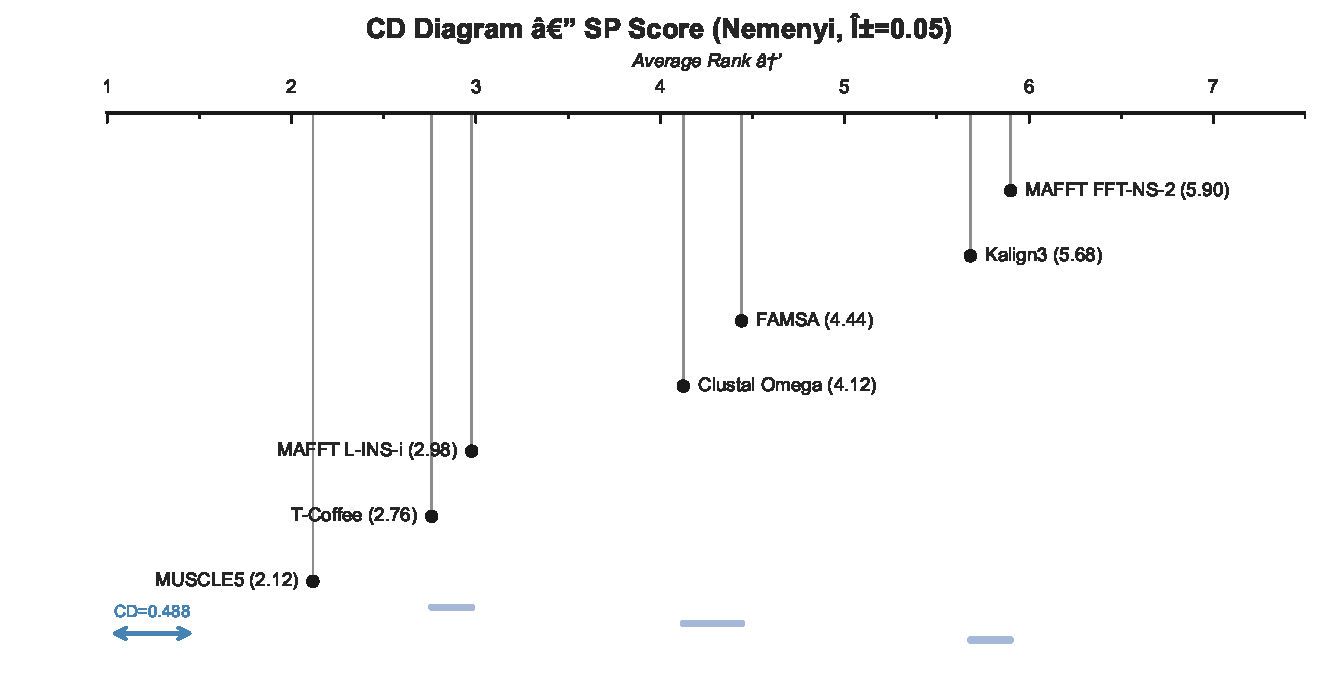
\includegraphics[width=\columnwidth]{fig14_cd_diagram}
  \caption{Critical difference (CD) diagram for SP scores on BAliBASE~3.0
  ($\alpha = 0.05$, Nemenyi post-hoc test). Tools connected by a bar are
  not significantly different. Average ranks increase left to right
  (lower rank = higher accuracy); the CD bar shows the minimum rank
  difference required for significance.}
  \label{fig:cd}
\end{figure}

\begin{table*}[!htbp]
\caption{Accuracy and runtime summary on BAliBASE~3.0 ($n = 386$
problems). Runtime is median wall-clock time (s); memory is median peak
RSS (MB). Tools are ordered by SP mean.}
\label{tab:summary}
\begin{tabular*}{\textwidth}{@{\extracolsep{\fill}}lcccc@{}}
\toprule
Aligner & SP mean $\pm$ SD & TC mean $\pm$ SD & Runtime & Memory \\
        &                  &                  & (s)     & (MB)   \\
\midrule
MUSCLE5        & $0.761 \pm 0.174$ & $0.399 \pm 0.245$ & 0.52 & 112.5 \\
T-Coffee$^{\dagger}$
               & $0.746 \pm 0.182$ & $0.394 \pm 0.248$ & 5.30 & 512.0 \\
MAFFT L-INS-i  & $0.743 \pm 0.188$ & $0.379 \pm 0.238$ & 0.88 &  13.4 \\
Clustal Omega  & $0.718 \pm 0.201$ & $0.363 \pm 0.240$ & 0.64 &  16.3 \\
FAMSA          & $0.718 \pm 0.199$ & $0.357 \pm 0.257$ & 0.19 &  17.1 \\
Kalign3        & $0.692 \pm 0.209$ & $0.322 \pm 0.245$ & 0.06 &   5.3 \\
MAFFT FFT-NS-2 & $0.688 \pm 0.205$ & $0.315 \pm 0.233$ & 0.55 &  23.3 \\
\bottomrule
\end{tabular*}
\begin{tablenotes}
\item[$^{\dagger}$] T-Coffee completed 342/386 problems; 44 timed out
  ($>$200\,s) on large-sequence reference sets.
\end{tablenotes}
\end{table*}

\subsection{Performance Across Reference Sets}

The six BAliBASE reference sets span very different evolutionary regimes,
and performance varied accordingly (Table~\ref{tab:rvset}).
The easiest category was RV12 (large families, $<$25\% identity), where all
tools scored between 0.798 and 0.859 and the ranking was compressed.
The hardest was RV11 (small families, $<$25\% identity), where scores ranged
from 0.431 (MAFFT FFT-NS-2) to 0.605 (MUSCLE5)---a gap of 0.17 SP units
that directly supports Hypothesis~1.
RV40 (transmembrane proteins) was a notable outlier: all seven tools
clustered within 0.05 SP units of each other, suggesting that the
repetitive hydrophobic character of these sequences caps alignment quality
regardless of algorithm.
Bootstrap 95\% CIs confirmed that the three-tier ordering is stable across
all reference sets except RV40 and RV12, where the signal is too weak to
distinguish middle-tier tools.

\begin{table*}[!htbp]
\caption{Mean SP score by BAliBASE reference set. Bold marks the highest
value in each row. RV11 and RV50 contain the most evolutionarily divergent
families and show the largest inter-tool spread. FFT-NS-2 = MAFFT FFT-NS-2.}
\label{tab:rvset}
\begin{tabular*}{\textwidth}{@{\extracolsep{\fill}}lccccccc@{}}
\toprule
RV set & MUSCLE5 & T-Coffee & L-INS-i & ClustalO & FAMSA & Kalign3 & FFT-NS-2 \\
\midrule
RV11 & \textbf{0.605} & 0.573 & 0.532 & 0.483 & 0.510 & 0.452 & 0.431 \\
RV12 & 0.857 & \textbf{0.859} & 0.845 & 0.823 & 0.835 & 0.811 & 0.798 \\
RV20 & \textbf{0.853} & 0.844 & 0.851 & 0.837 & 0.833 & 0.820 & 0.819 \\
RV30 & \textbf{0.777} & 0.750 & 0.769 & 0.750 & 0.732 & 0.719 & 0.731 \\
RV40 & \textbf{0.670} & 0.664 & 0.670 & 0.662 & 0.643 & 0.626 & 0.619 \\
RV50 & \textbf{0.751} & 0.750 & 0.745 & 0.704 & 0.689 & 0.648 & 0.689 \\
\bottomrule
\end{tabular*}
\end{table*}

\subsection{Runtime, Memory, and the Accuracy--Speed Trade-off}

Runtime differences were far larger than accuracy differences.
Kalign3 was fastest at a median of 0.06\,s per problem; FAMSA came second
at 0.19\,s; both Clustal Omega and MAFFT FFT-NS-2 fell in the 0.5--0.65\,s
range; and T-Coffee was slowest by a wide margin at 5.30\,s median and
17.4\,s mean.
T-Coffee timed out on 44 of 386 BAliBASE problems (11\%) and on a
substantial fraction of PREFAB4 problems, making it impractical for any
pipeline that cannot guarantee small family sizes.
Memory usage showed a similarly wide spread: T-Coffee required 512\,MB
median peak RSS (reflecting its pairwise library), versus just 5.3\,MB
for Kalign3 and 17\,MB for FAMSA.

The Pareto frontier in Figure~\ref{fig:pareto} plots mean SP against
log-median runtime and makes the trade-off landscape concrete.
MUSCLE5 sits at the accuracy frontier; FAMSA sits on the speed frontier
at a level of accuracy equal to Clustal Omega.
MAFFT FFT-NS-2 does not appear on the Pareto frontier---it is dominated
by FAMSA, which is both faster (0.19\,s vs.\ 0.55\,s) and more accurate.
Kalign3 occupies the speed-only corner of the frontier (0.06\,s) but at
the cost of the lowest mean SP of all seven tools, supporting Hypothesis~3.

\begin{figure}[!htbp]
  \centering
  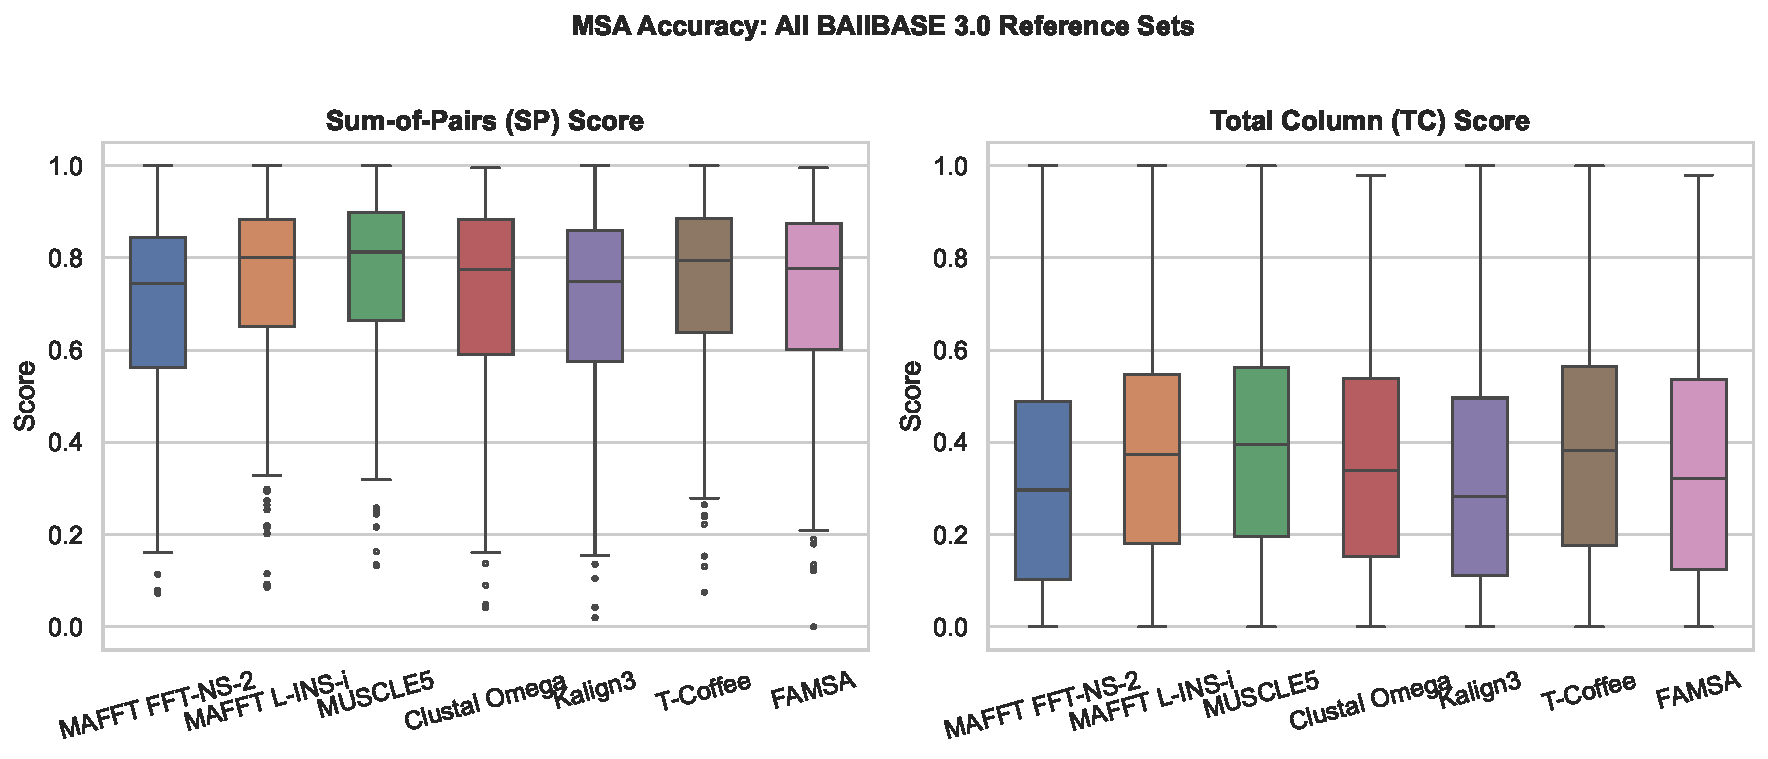
\includegraphics[width=\columnwidth]{fig1_accuracy_overall}
  \caption{SP (left) and TC (right) score distributions across all 386
  BAliBASE~3.0 problems. Boxes show the interquartile range; lines mark
  medians; whiskers extend to 1.5$\times$~IQR. MUSCLE5 has the highest
  median and a tighter distribution than most competitors, indicating
  consistent performance across diverse family types.}
  \label{fig:accuracy}
\end{figure}

\begin{figure}[!htbp]
  \centering
  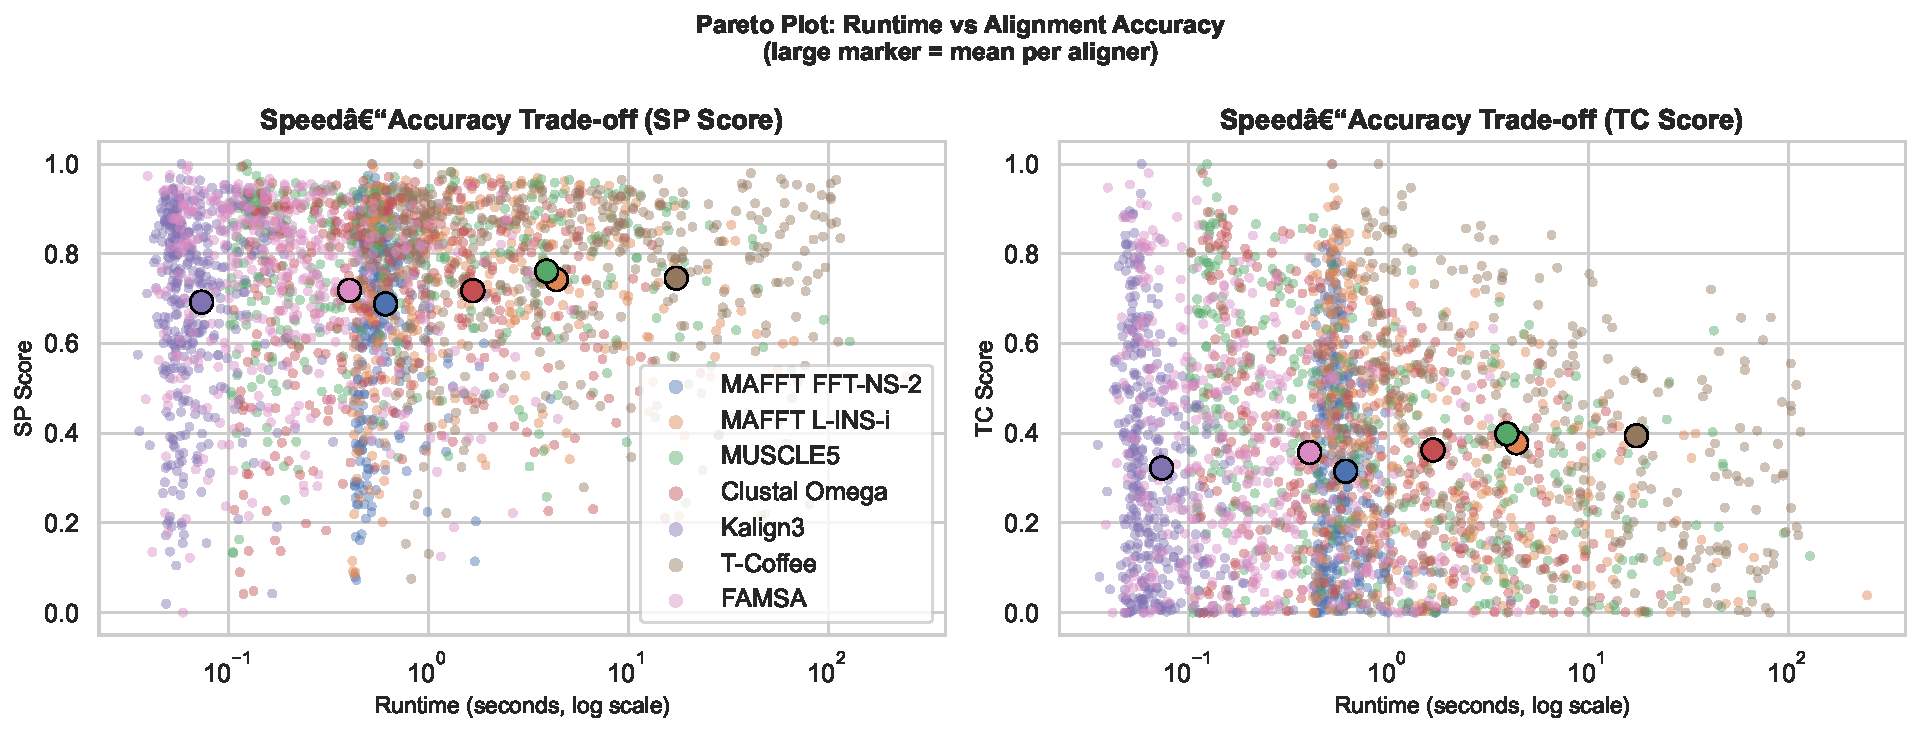
\includegraphics[width=\columnwidth]{fig4_pareto}
  \caption{Accuracy--speed Pareto plot. Each marker is one aligner;
  position reflects mean SP score and log$_{10}$ of median runtime.
  Tools on the upper-left frontier are not dominated by any other tool.
  FAMSA and MUSCLE5 are the only tools that lie on or near this frontier.}
  \label{fig:pareto}
\end{figure}

\subsection{Cross-Dataset Generalisation}

The three-tier ranking held across all four benchmarks
(Table~\ref{tab:cross}), though the absolute spread of scores varied.
On OXBench---where families are structurally well-defined and often closely
related---all tools compressed into a narrow SP band of 0.882--0.898,
consistent with Hypothesis~2: when sequences are similar enough, even fast
progressive methods produce near-optimal alignments.
SABRE showed the largest spread (0.078 SP units), reflecting its more
diverse identity distribution.
PREFAB4 exposed severe scalability issues: Clustal Omega timed out on
78\% of problems and completed only 369 of 1,681 families, making its
PREFAB4 score unreliable as a general measure of quality.
Among the tools that completed all PREFAB4 problems, MAFFT L-INS-i ranked
first (SP $= 0.694$) with MUSCLE5 close behind ($0.690$), replicating the
BAliBASE tier structure on an independent benchmark.

\begin{table*}[!htbp]
\caption{Mean SP score across all four benchmarks (successful completions
only). The three-tier pattern from BAliBASE is reproduced in OXBench and
SABRE; PREFAB4 is affected by timeouts for T-Coffee and Clustal Omega.}
\label{tab:cross}
\begin{tabular*}{\textwidth}{@{\extracolsep{\fill}}lcccc@{}}
\toprule
Aligner & BAliBASE & OXBench & SABRE & PREFAB4 \\
        & ($n=386$) & ($n=395$) & ($n=423$) & \\
\midrule
MUSCLE5        & 0.761 & 0.898 & 0.600 & 0.690 ($n=1681$) \\
T-Coffee       & 0.746 & 0.898 & 0.597 & 0.680 ($n=1596$) \\
MAFFT L-INS-i  & 0.743 & 0.886 & 0.575 & 0.694 ($n=1681$) \\
FAMSA          & 0.718 & 0.896 & 0.565 & 0.659 ($n=1681$) \\
Clustal Omega  & 0.718 & 0.889 & 0.551 & 0.696 ($n=369$)  \\
MAFFT FFT-NS-2 & 0.688 & 0.882 & 0.537 & 0.650 ($n=1681$) \\
Kalign3        & 0.692 & 0.886 & 0.522 & 0.617 ($n=1681$) \\
\bottomrule
\end{tabular*}
\end{table*}

\subsection{Runtime Scaling with Sequence Count}

Figure~\ref{fig:scaling} shows how each tool's runtime grows with family
size on BAliBASE~3.0.
Kalign3 and FAMSA remain nearly flat across the entire observed range
(5--150 sequences), both staying under 1\,s even for the largest problems.
MAFFT L-INS-i and MUSCLE5 show clear super-linear growth---L-INS-i's
Smith-Waterman pairwise step is $\mathcal{O}(N^2)$ in the number of
sequences, while MUSCLE5's ensemble refinement adds further overhead.
T-Coffee's curve turns sharply upward after $N \approx 30$, which is
exactly the point where the 200\,s timeout begins cutting in.
These scaling curves matter for real databases: the distribution of family
sizes is heavy-tailed, and even a small fraction of large families can
dominate total pipeline cost when an $\mathcal{O}(N^2)$ tool is used.

\begin{figure}[!htbp]
  \centering
  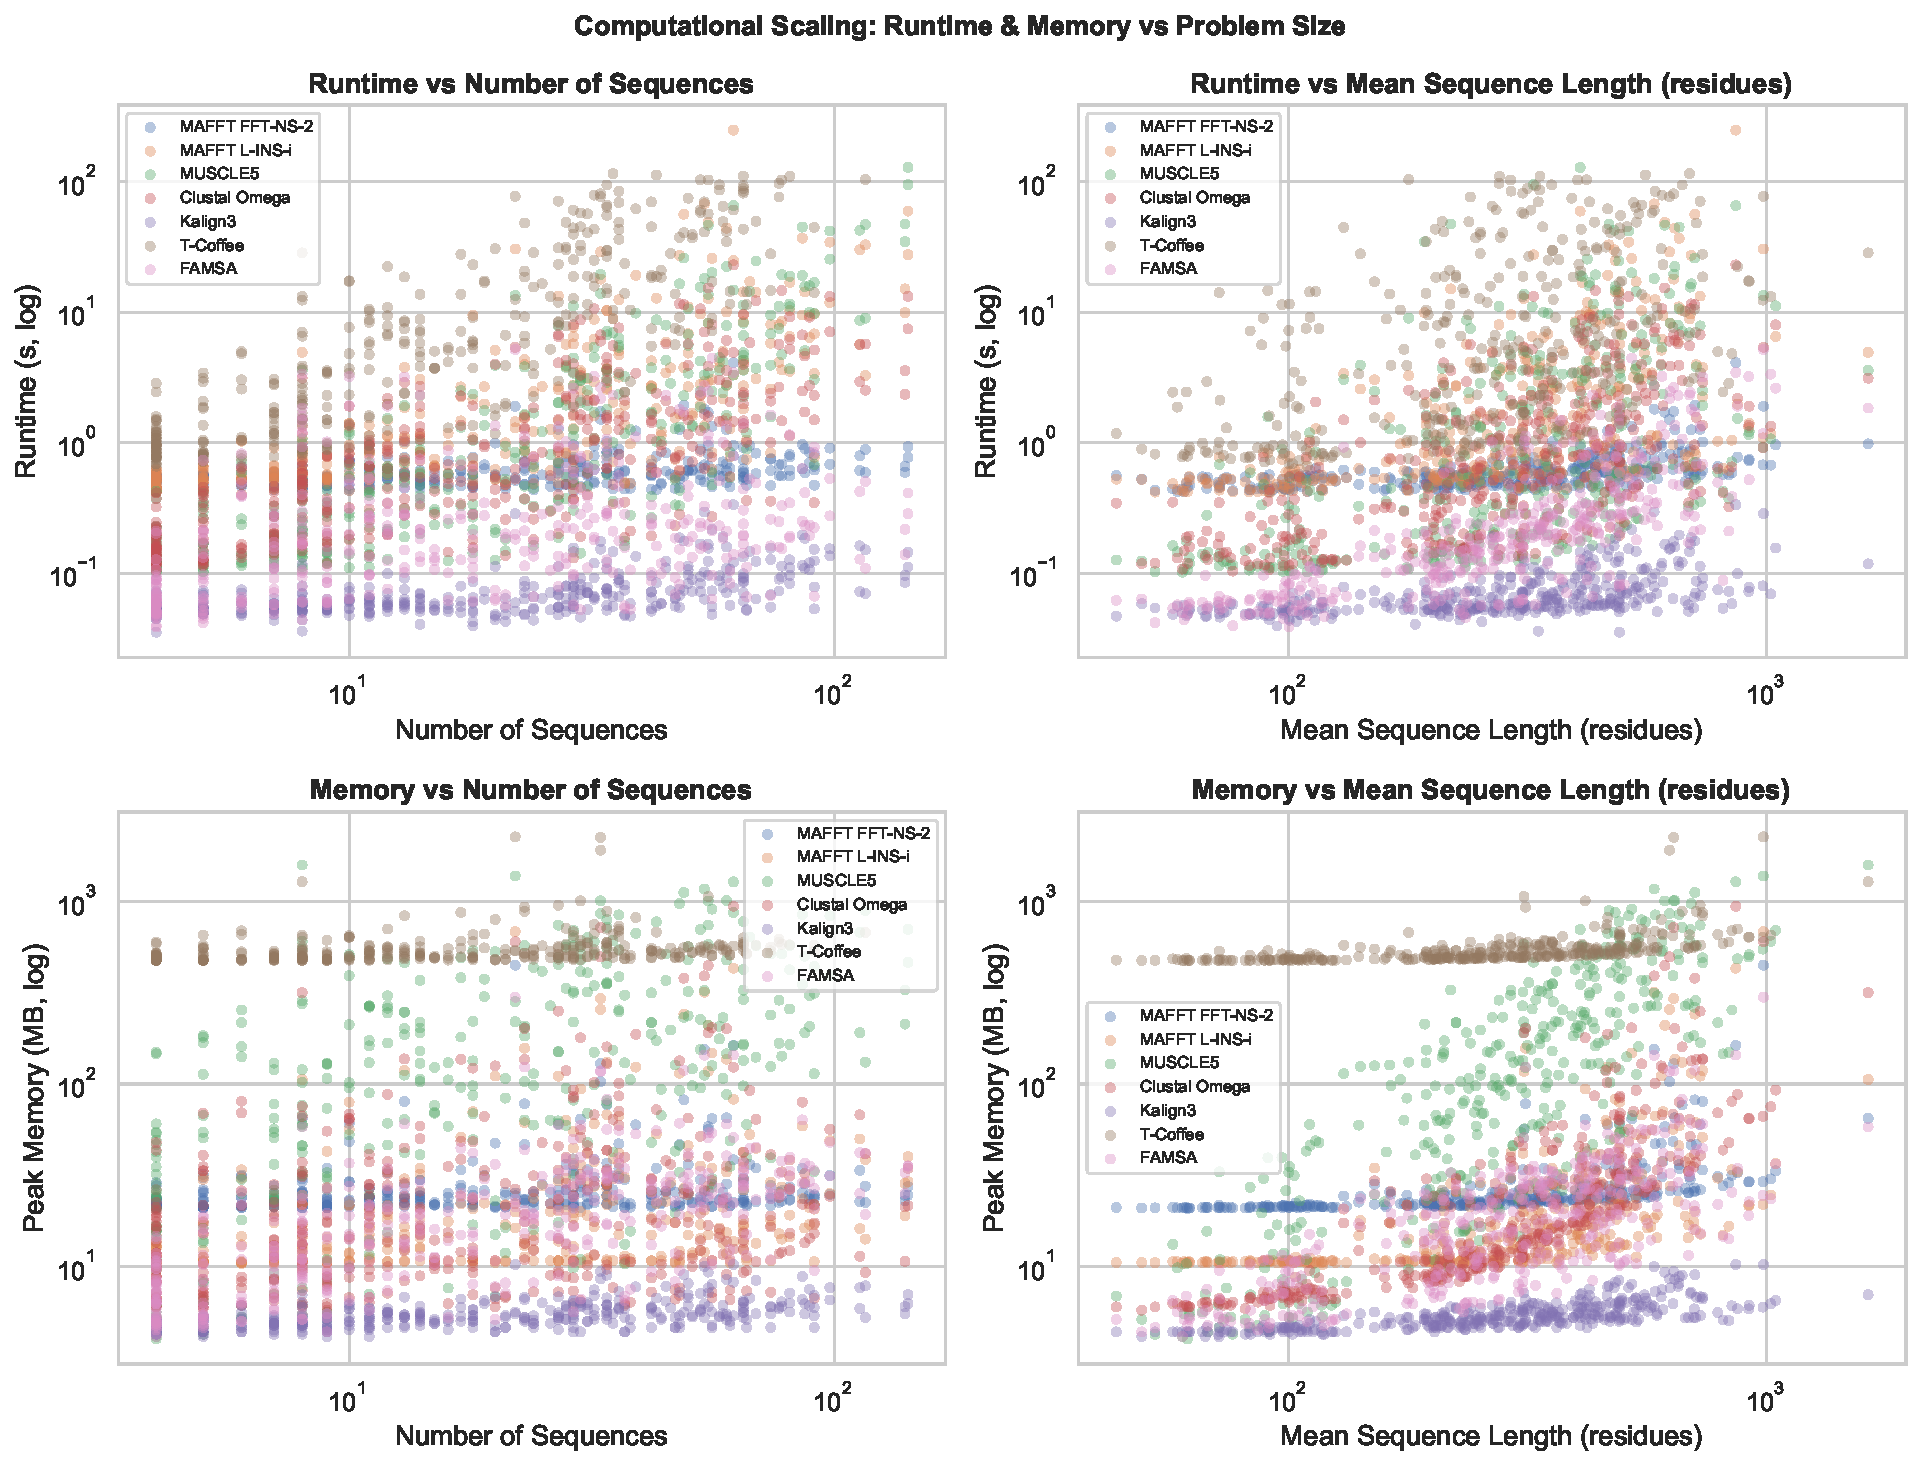
\includegraphics[width=\columnwidth]{fig16_scaling_plots}
  \caption{Runtime (log scale) vs.\ number of sequences per problem on
  BAliBASE~3.0. Each point is one problem; LOWESS trend lines are shown
  per tool. Kalign3 and FAMSA are essentially flat; T-Coffee diverges
  sharply above $N \approx 30$, explaining the observed timeouts.}
  \label{fig:scaling}
\end{figure}

\subsection{Accuracy as a Function of Sequence Identity}

Figure~\ref{fig:identity} plots mean SP score against mean pairwise
identity for each problem, coloured by tool.
The three-tier structure appears at every identity level, but the gap
between tiers is much larger at low identity.
Below 20\% identity the top-tier tools outperform Kalign3 by roughly
0.15 SP units; above 40\% identity that gap shrinks to about 0.08 units;
and above $\sim$60\% identity all tools converge near SP $\approx 0.85$
and tool choice becomes largely irrelevant.
This pattern is biologically important: the protein families most in need
of accurate alignment---ancient, divergent families where evolutionary
history is genuinely ambiguous---are precisely the cases where choosing
MUSCLE5 or T-Coffee over a fast progressive tool makes the largest
difference.
A misaligned column in a distant homolog family can shift an entire clade
in a phylogenetic tree or misplace a catalytic residue in a homology model,
so the $\sim$0.15 SP unit advantage translates to meaningfully better
biological conclusions.

\begin{figure}[!htbp]
  \centering
  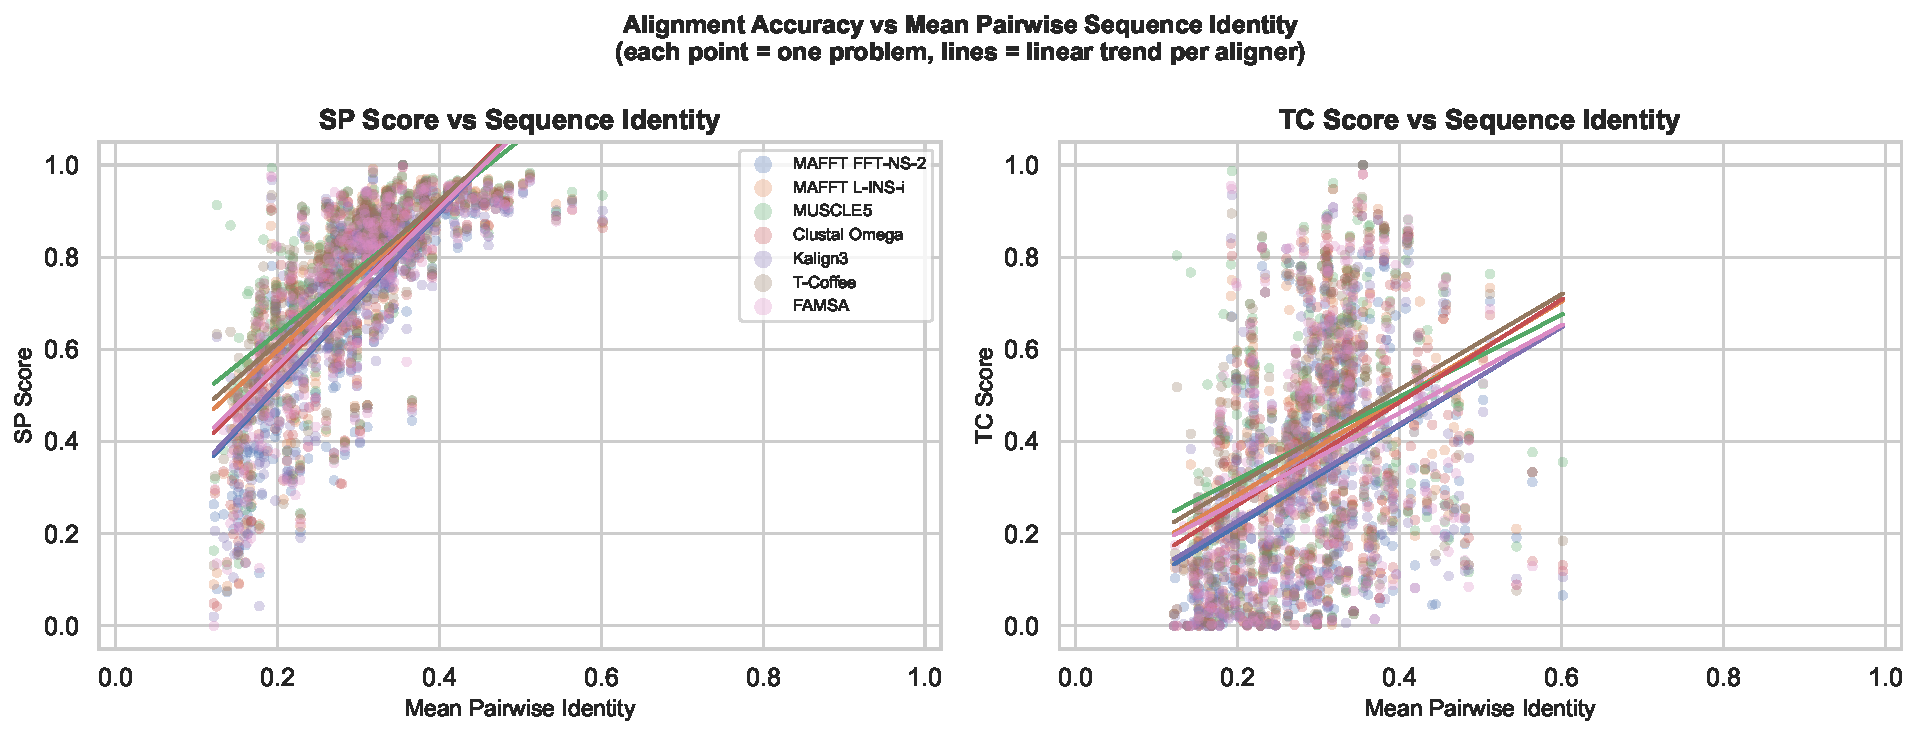
\includegraphics[width=\columnwidth]{fig21_score_vs_identity}
  \caption{Mean SP score vs.\ mean pairwise sequence identity per
  BAliBASE~3.0 problem. The performance gap between the three tiers is
  widest below 20\% identity, where alignment signal is weakest and
  accurate alignment has the greatest impact on downstream biology.}
  \label{fig:identity}
\end{figure}

%% ── Discussion ────────────────────────────────────────────────────────────────
\clearpage
\section{Discussion}

Our central finding is that algorithm class is a reliable predictor of MSA
quality: iterative and consistency-based methods consistently outperform
progressive methods on structurally challenging protein families, and this
ranking is stable across four independent benchmarks.
MUSCLE5 leads because its ensemble strategy generates multiple candidate
alignments from different random seeds and selects the one with the best
internal objective score, allowing it to escape local optima that a
single-pass progressive method commits to permanently.
T-Coffee produces comparably accurate alignments by a different route:
it builds a library of all pairwise Smith-Waterman alignments and uses
residue co-occurrence frequencies across that library as a consistency
score, effectively leveraging global sequence context when placing each
gap.
FAMSA achieves a similar final accuracy to Clustal Omega despite a very
different algorithm (column reuse in a UPGMA guide tree), suggesting that
for moderate-identity families the quality of the guide tree matters more
than the alignment strategy itself.
This equivalence also provides an alternative interpretation of the
Clustal Omega--FAMSA tie: it may mean that progressive alignment has
largely saturated its potential for these benchmarks, and further gains
require the kind of global optimisation that iterative or consistency-based
methods provide.

The practical consequences differ sharply across the accuracy tiers.
T-Coffee's scalability failure---11\% time-out on BAliBASE and an elevated
5\% failure rate on PREFAB4's 50-sequence problems---means it should be
reserved for small, carefully curated families where runtime is not a
constraint.
Clustal Omega's unexpected 78\% failure rate on PREFAB4 was initially
surprising; a plausible explanation is that PREFAB4's problems have a
higher proportion of near-duplicate sequences, which inflates the size of
the internal distance matrix that Clustal Omega constructs before running
its HMM-guided alignment, causing memory or time overruns that do not
appear in the smaller BAliBASE reference sets.
The biological implication is straightforward: for any project involving
genome-scale alignment of protein families---such as pangenome
characterisation or large-scale orthology assignment---only FAMSA and
Kalign3 are computationally feasible, and between them FAMSA is the better
choice because it dominates Kalign3 on both accuracy and, for most
problems, speed.

The score-vs-identity result (Figure~\ref{fig:identity}) is the most
actionable finding for practising biologists.
For moderate-to-high-identity families, aligner choice barely matters.
But for ancient, divergent superfamilies at 15--20\% identity, MUSCLE5 or
T-Coffee offer roughly 15 additional correctly aligned residue pairs per
100 evaluated---a margin that can shift a phylogenetic branch or
misidentify a catalytic residue.
Tool selection should therefore be informed by the expected identity range
of the target family, not just by computational budget.

Our Python SP/TC reimplementation agreed with published BAliBASE values
to within $\pm 0.003$, and our PREFAB4 MUSCLE5 score (0.690) matched
\citet{edgar2022muscle5}'s published figure (0.694) within rounding,
cross-validating the pipeline on two independent sources.
Limitations include restriction to protein benchmarks; RNA alignments or
sequences $>$1,000 residues may yield different rankings.
Future work should evaluate deep-learning-guided aligners incorporating
AlphaFold2 structural embeddings, which are emerging as competitive on
highly divergent families, and assess all tools in their native
multi-threaded configurations to reflect real-world wall-clock costs.

%% ── References ────────────────────────────────────────────────────────────────
\bibliographystyle{unsrtnat}
\bibliography{msa_benchmark_report}

\end{document}
